\documentclass[12pt, a4paper]{article}

\usepackage[utf8]{inputenc}
\usepackage[T1]{fontenc}
\usepackage{mathptmx}
\usepackage[margin=1in]{geometry}
\usepackage{graphicx}
\usepackage{booktabs}
\usepackage{amsmath}
\usepackage{amssymb}
\usepackage{hyperref}
\usepackage{natbib}
\usepackage{caption}
\captionsetup{font=small}
\usepackage{subcaption}
\usepackage{float}
\usepackage{xcolor}
\usepackage{setspace}
\usepackage{titlesec}
\usepackage{placeins}
\titleformat{\section}{\normalsize\bfseries}{\thesection}{1em}{}
\titleformat{\subsection}{\normalsize\bfseries}{\thesubsection}{1em}{}
\titleformat{\subsubsection}{\normalsize\bfseries}{\thesubsubsection}{1em}{}
\titlespacing*{\section}{0pt}{12pt}{6pt}
\titlespacing*{\subsection}{0pt}{10pt}{4pt}
\titlespacing*{\subsubsection}{0pt}{8pt}{4pt}

\hypersetup{
    colorlinks=true,
    linkcolor=blue!70!black,
    citecolor=blue!70!black,
    urlcolor=blue!70!black
}

\onehalfspacing

\setlength{\intextsep}{4pt plus 2pt minus 2pt}
\setlength{\floatsep}{4pt plus 2pt minus 2pt}
\setlength{\textfloatsep}{6pt plus 2pt minus 4pt}
\setlength{\abovecaptionskip}{4pt}
\setlength{\belowcaptionskip}{2pt}
\renewcommand{\topfraction}{0.9}
\renewcommand{\bottomfraction}{0.9}
\renewcommand{\textfraction}{0.1}
\renewcommand{\floatpagefraction}{0.8}
\setcounter{topnumber}{3}
\setcounter{bottomnumber}{3}
\setcounter{totalnumber}{5}

\title{\textbf{The Geometry of Gridlock: Tracking Congressional Polarization\\ Through Spectral Analysis of Co-Voting Networks}}

\author{Jacob Crainic}

\date{}

\begin{document}
\raggedbottom

\maketitle

\begin{abstract}
Congressional polarization is typically measured by placing legislators on an ideological spectrum, but this approach misses the relational structure of legislative cooperation. We construct co-voting networks for every U.S.\ House Congress from the 100th (1987) through the 118th (2025), connecting legislators who agree on a majority of shared roll-call votes, and track their spectral properties over time. The algebraic connectivity of these networks, measured by the Fiedler value, rises from 0.534 in the 100th Congress to a peak of 0.805 in the post-9/11 107th Congress, surges again to 0.737 in the 111th Congress (Obama supermajority), then collapses to 0.032 by the 118th, indicating near-complete structural disconnection between partisan blocs. Though the magnitudes of the mid-period spikes are attenuated when restricted to substantive policy votes (excluding near-unanimous suspension bills), the post-2010 collapse is robust across all vote subsets. The 111th-to-112th transition, coinciding with the Tea Party wave, represents a Fiedler decline of 0.664, the single largest congress-to-congress structural shock in the dataset. An analysis of structural recovery reveals that the network's capacity to absorb and recover from shocks has itself deteriorated: the post-Contract with America period produced full structural recovery, while the post-2010 collapse proved permanent. We introduce a Bridge Legislator Index quantifying each member's contribution to network connectivity. GEE regression shows that BLI predicts congressional departure ($\beta = 180.2$, $p < 10^{-7}$) beyond ideology distance, seniority, and party affiliation, with a significant partisan asymmetry ($\text{BLI} \times \text{Republican}$ interaction, $p = 0.018$); however, this effect is substantially attenuated when controlling for absolute ideological centrism ($p = 0.30$), indicating that the electoral vulnerability of bridge legislators operates primarily through their moderate positioning rather than their network role per se. Null model comparisons against degree-preserving configuration models and a linear-decline temporal model confirm that the oscillatory pattern is genuinely structural, not a mechanical consequence of shifting degree distributions. Counterfactual perturbation experiments suggest that the structural difference between the connected 103rd Congress and the disconnected 118th can be accounted for under our perturbation assumptions by the presence or absence of on the order of 35 bridge legislators. These findings reframe polarization as a topological phenomenon and suggest that the structural scaffolding of bipartisan cooperation has lost its capacity for self-repair.
\end{abstract}

\section{Introduction}

In October 2013, the Affordable Care Act had been law for three years. It had survived a Supreme Court challenge, a presidential election, and forty-two separate repeal votes in the House of Representatives. And yet, on October 1, a faction of House Republicans refused to fund the government unless the law was defunded, triggering a sixteen-day shutdown that furloughed 800,000 federal employees and cost the economy an estimated \$24 billion \citep{cbo2013}. The vote that ended it split almost perfectly along party lines.

That shutdown reflected a deeper structural transformation. Over the preceding two decades, the U.S. Congress had undergone a transformation so thorough that it altered the basic structure of legislative cooperation. Members who once voted across party lines with some regularity stopped doing so. The moderate center of both parties hollowed out. By the 114th Congress (2015--2017), the most liberal Republican in the House was more conservative than the most conservative Democrat, a pattern with no precedent in the modern era \citep{poole2017}.

The standard way to measure this shift is DW-NOMINATE, a scaling method that places legislators on an ideological spectrum based on their roll-call votes \citep{poole1985}. It works well for what it does. But it treats each legislator as an independent point in ideological space, missing something that anyone who has watched Congress closely can feel: polarization concerns how legislators cluster, who cooperates with whom, and how those cooperative structures have fractured over time.

We take a different approach here. Instead of placing legislators on a line, we place them in a network. For each Congress from the 100th through the 118th, we construct a co-voting graph where edges connect members who agree on roll-call votes above a threshold. What happens to these networks over time is stark. The algebraic connectivity of the House co-voting network, a spectral measure of how tightly connected the graph is, rose from 0.534 in 1987 to a peak of 0.805 in the post-9/11 107th Congress, surged again to 0.737 during the Obama supermajority (111th), then collapsed to 0.032 by 2023. The trajectory is non-monotonic, and the non-monotonicity is one of our key findings: the graph did not simply erode over time but rather surged in connectivity before fracturing. These mid-period spikes are partially inflated by near-unanimous suspension votes; on substantive policy votes alone, the peaks are smaller but the overall oscillatory pattern persists, validated by null model comparisons (Section~4). The single largest congress-to-congress collapse, a Fiedler decline of 0.664 between the 111th and 112th Congresses, coincided with the Tea Party wave of 2010. By the 118th Congress, the network had effectively split in two.

This paper makes three contributions. First, we present the longest spectral analysis of congressional co-voting networks to date: 19 Congresses spanning 36 years, revealing a previously undocumented oscillatory pattern in network connectivity that ideological scaling methods entirely miss. Second, we introduce a Bridge Legislator Index that quantifies individual members' contributions to network connectivity. GEE regression on 7,500 member-congress observations shows that bridge position predicts congressional departure ($p < 10^{-7}$) beyond ideology distance, seniority, and party, though the effect is largely attributable to the ideological centrism of bridge legislators rather than a distinct network mechanism (Section~8). Third, we formalize the asymmetry between the post-9/11 recovery and the post-Tea Party stagnation through a structural recovery analysis showing that the network's capacity to absorb perturbations has itself deteriorated across successive shocks.

\section{Related Work}

The dominant framework for measuring legislative ideology is DW-NOMINATE, a spatial scaling method that places legislators on a left-right continuum based on their roll-call votes \citep{poole1985, poole2017}. It has been enormously productive: the divergence of the two parties since the 1970s is among the most robust findings in American politics. But NOMINATE is fundamentally a spatial model. It embeds legislators as independent points and votes as cutting lines, capturing ideological position while discarding the relational structure of who cooperates with whom.

Recognizing this limitation, a network-analytic literature emerged in the early 2000s. \citet{fowler2006a} constructed co-sponsorship networks and found that legislative connectedness predicts bill passage. \citet{waugh2009} applied modularity measures to co-voting networks and documented increasing partisan clustering over time. \citet{andris2015} produced striking visualizations of the near-complete disappearance of cross-party edges between the 1980s and 2010s. These contributions established that network structure carries information beyond what spatial models capture. What remained missing was a formal framework connecting network topology to the mechanisms of polarization: the specific structural features that degrade, the members whose removal matters most, and the system's capacity to recover from shocks.

Spectral graph theory offers tools suited to this task. The Fiedler value, the second-smallest eigenvalue of the graph Laplacian, measures how close a network is to splitting into disconnected components \citep{fiedler1973}. \citet{newman2006} used spectral methods to identify partisan structure in congressional networks, and \citet{moody2013} traced the evolution of partisan clustering with related techniques. Our analysis extends this spectral tradition with a substantially longer time series, a novel node-level centrality measure grounded in the Fiedler value, and a formal statistical test linking bridge position to electoral vulnerability.

A natural alternative to spectral methods is stochastic block modeling (SBM), which identifies latent community structure from network data. In congressional networks, however, SBMs trivially recover party labels as the dominant partition. Our interest is not in detecting communities---which are known a priori---but in measuring the \textit{connectivity between} known communities, which is precisely what the Fiedler value captures. The BLI has no natural SBM analog: it measures individual contribution to inter-community connectivity rather than community membership probability. We therefore position spectral analysis as complementary to SBMs rather than competing with them.

On the political science side, \citet{theriault2008} documented how procedural changes accelerated partisan conflict, \citet{skocpol2012} analyzed the Tea Party as both grassroots movement and elite-driven realignment, and \citet{mann2012} argued that asymmetric polarization driven by the Republican Party's rightward shift is the dominant dynamic. These accounts offer complementary causal narratives. Our spectral time series and structural recovery analysis provide an independent, network-structural test of when and how sharply the cooperative architecture of Congress fractured, and whether the fractures proved reversible.

\section{Data and Graph Construction}

\subsection{Roll-Call Voting Records}

Roll-call voting records come from Voteview \citep{lewis2023}, covering the U.S. House of Representatives from the 100th Congress (1987--1989) through the 118th Congress (2023--2025). Each record indicates whether a member voted yea, nay, or did not vote. We filter to members affiliated with the two major parties and require a minimum of 50 recorded votes per member. This yields an average of 442 members per Congress across 19 Congresses, or approximately 8,400 member-Congress observations.

\subsection{Co-Voting Agreement Networks}

For each pair of members within a Congress, we compute a pairwise agreement score as the fraction of shared roll calls on which both cast the same vote. For members $i$ and $j$ who both voted on roll calls $\mathcal{R}_{ij}$:
\begin{equation}
    a_{ij} = \frac{|\{r \in \mathcal{R}_{ij} : v_i^r = v_j^r\}|}{|\mathcal{R}_{ij}|}
\end{equation}
where $v_i^r \in \{0, 1\}$ denotes the vote of member $i$ on roll call $r$. We require $|\mathcal{R}_{ij}| \geq 20$.

The agreement matrix $A$ is dense. Many votes are near-unanimous. We threshold at $\tau = 0.5$ to create an unweighted adjacency matrix $\hat{A}$ where an edge indicates agreement on a majority of shared votes. While we report our primary findings using an unweighted binary agreement threshold of $\tau = 0.5$ to establish clear topological boundaries, our findings regarding the collapse of the algebraic connectivity are not artifacts of this specific cutoff. The qualitative pattern of the Fiedler value deterioration remains highly stable across agreement thresholds ranging from $\tau = 0.4$ to $0.7$, as detailed in the sensitivity analysis in Appendix~\ref{app:threshold}.

\subsection{Node Features}

Each node has an eight-dimensional feature vector: DW-NOMINATE scores on both dimensions \citep{poole2017}, party affiliation, vote participation rate, yea-vote rate, mean agreement with all other members, mean cross-party agreement, and mean within-party agreement. These features characterize each legislator's voting profile and position within the co-voting network. In the departure analysis (Section~8), we use ideology scores, party affiliation, and seniority as covariates; the agreement-based features enter implicitly through the BLI, which is computed from the adjacency matrix they help define.

\section{Spectral Analysis}

\subsection{Algebraic Connectivity and Polarization}

The normalized graph Laplacian is $L = I - D^{-1/2} \hat{A} D^{-1/2}$, where $D$ is the diagonal degree matrix. Its second-smallest eigenvalue, the Fiedler value $\lambda_2$, measures how well-connected the graph is. Values near zero indicate the graph is close to splitting into disconnected components; larger values indicate a more integrated structure \citep{fiedler1973}.

In the 100th Congress (1987), $\lambda_2$ stood at 0.534. By the 114th (2015), it had fallen to 0.010, a decline of over 98\%. The co-voting graph had, in structural terms, nearly split in two. Table~\ref{tab:polarization} summarizes these metrics across the study period.

\begin{table}[H]
\centering
\caption{Congressional polarization metrics across selected Congresses. The Fiedler value captures network connectivity; party distance measures ideological divergence. Both deteriorate, but at different rates and with different dynamics. The 111th Congress row is new to this analysis and reveals a previously undocumented connectivity spike.}
\label{tab:polarization}
\begin{tabular}{lcccccc}
\toprule
Congress & Years & Members & Fiedler & Party Dist. & Density & Mean Degree \\
\midrule
100th & 1987--89 & 439 & 0.534 & 0.666 & 0.780 & 341.6 \\
103rd & 1993--95 & 441 & 0.230 & 0.712 & 0.609 & 268.1 \\
107th & 2001--03 & 439 & 0.805 & 0.786 & 0.928 & 406.5 \\
111th & 2009--11 & 450 & 0.737 & 0.794 & 0.897 & 402.8 \\
112th & 2011--13 & 442 & 0.073 & 0.867 & 0.538 & 237.4 \\
114th & 2015--17 & 436 & 0.010 & 0.886 & 0.512 & 222.9 \\
117th & 2021--23 & 447 & 0.086 & 0.880 & 0.536 & 238.8 \\
118th & 2023--25 & 451 & 0.032 & 0.892 & 0.510 & 229.3 \\
\bottomrule
\end{tabular}
\end{table}

\subsection{Density Without Connectivity}

Density declines only modestly from 0.780 to 0.510 even as the Fiedler value collapses from 0.534 to 0.010 (Table~\ref{tab:polarization}). This disproportionality reveals that edges are not simply lost but reorganized: within-party connections densify while cross-party bridges vanish. The network retains most of its edges even as it structurally fractures. Polarization is a structural rewiring, not a loss of cooperation, and aggregate measures like density miss this entirely.

\subsection{Validation Against DW-NOMINATE}

The Fiedler value and DW-NOMINATE party distance both capture polarization, but they are not the same measure. Party distance tracks the separation between mean ideological positions; the Fiedler value tracks structural connectivity of the cooperation network. They correlate ($r = -0.76$, since lower Fiedler means more polarized), but the dynamics differ (Figure~\ref{fig:polarization}).

The most visible difference: the Fiedler value shows a sharp, non-monotonic trajectory. It rises from 0.534 in the 100th Congress to 0.805 in the 107th (2001--2003), then falls, surges again to 0.737 in the 111th (2009--2011), and collapses to near zero by the 113th. Party distance, by contrast, increases smoothly and monotonically. The network structure captures dynamics that ideological scaling misses: temporary surges in bipartisan cooperation and sudden structural breaks that get smoothed away in spatial models.

The 107th Congress deserves attention. A Fiedler value of 0.805 represents the most structurally connected House in our entire dataset, and it occurred when DW-NOMINATE party distance was already high (0.786). The explanation lies substantially in the post-9/11 rally effect: the Authorization for Use of Military Force passed the House 420--1, and a wave of national security legislation drew broad bipartisan support that temporarily rewired the co-voting graph. An important caveat: when restricted to substantive policy votes---excluding procedural motions and near-unanimous suspension bills---the 107th's Fiedler value drops from 0.805 to 0.210 (Appendix~\ref{app:vote_filter}). The post-9/11 cooperation surge was real but partially concentrated in suspension votes, which are bipartisan by design. The exogenous shock still produced a genuine structural deviation from the temporal null (Section~4.4), but the spike's magnitude on contested legislation was considerably more modest.

The 111th Congress (2009--2011) reveals a second connectivity spike. With a Fiedler value of 0.737 on all votes (0.110 on substantive votes only), the Obama supermajority Congress shows elevated bipartisan cooperation, again concentrated in suspension and procedural categories. The mechanism is not entirely clear. TARP was enacted in the 110th Congress (October 2008), not the 111th, and the Affordable Care Act passed on a party-line vote. One plausible explanation is that the large Democratic majority allowed conservative Democrats to defect on high-profile bills without endangering passage, creating cross-party voting patterns with Republicans on fiscal and defense legislation. Whatever the cause, the result on the full vote set is a striking oscillation: the Fiedler value swings from 0.238 (110th) to 0.737 (111th) to 0.073 (112th), a range of 0.664 in just two transitions. On substantive votes the oscillation is smaller (0.073 to 0.110 to 0.036) but the post-Tea Party collapse is, if anything, starker. The Tea Party wave did not merely continue a gradual decline; it shattered even the modest substantive cooperation that remained.

What happened after each connectivity peak is the key finding. The post-9/11 surge reversed within two Congresses, with the Fiedler value falling from 0.805 back below 0.5 by the 109th. The system snapped back. Now compare that to the post-2010 period: after the Tea Party wave drove connectivity from 0.737 to 0.073, no subsequent event produced anything resembling a recovery. Not the Trump presidency, not the January 6th crisis, not a global pandemic. The graph stayed disconnected. This asymmetry points to something beyond the level of polarization itself. In the early 2000s, a crisis could temporarily override partisan sorting and rebuild bipartisan cooperation. By the 2010s, that capacity appears to have been lost. The network cannot regenerate the cross-party connections that crises once produced.

\subsection{Null Model Validation}

To test whether the observed Fiedler trajectory reflects genuine partisan structure rather than a mechanical consequence of shifting degree distributions, we compare the empirical values against two null models (Figure~\ref{fig:nullmodel}).

The first null preserves each Congress's degree sequence via the configuration model: for each of the 19 Congresses, we generate 1,000 random graphs with the same degree sequence and compute the Fiedler value for each. The configuration model null produces Fiedler values tightly concentrated around 0.90 for all Congresses (95\% CI: approximately $[0.885, 0.926]$ across the dataset). Every empirical Fiedler value falls far below this band ($p < 0.001$ for all 19 Congresses), confirming that the observed connectivity levels cannot be explained by degree distributions alone. The partisan segregation of edges---not the number of edges per member---drives the low algebraic connectivity.

The second null tests whether the non-monotonicity is surprising given the overall decline in cross-party cooperation. We fit a linear model to the observed aggregate cross-party agreement rate (slope $= -0.012$ per Congress) and, for each Congress, simulate 200 networks where cross-party agreement follows the predicted linear decline with Gaussian noise. The resulting Fiedler trajectory declines monotonically. Critically, the empirical Fiedler values for the 106th through 111th Congresses exceed the temporal null's upper 95\% confidence bound, confirming that the post-9/11 and Obama-era connectivity spikes represent genuine structural deviations from trend rather than noise. A linear decline model cannot reproduce these oscillations. Conversely, the post-112th collapse is consistent with the temporal null's prediction of near-zero connectivity, suggesting that the system's endpoint is in line with the overall trend even if the path to it was not.

\begin{figure}[H]
    \centering
    \includegraphics[width=\textwidth]{paper_figures/null_model_band.pdf}
    \caption{Empirical Fiedler trajectory against two null models. Gray band: 95\% CI from 1,000 configuration model random graphs per Congress (degree-preserving). Orange dotted: linear-decline temporal null. All empirical values fall far below the configuration model band, confirming that partisan edge segregation, not degree distribution, drives low connectivity. The 106th--111th empirical values exceed the temporal null, validating the non-monotonic oscillation as structurally genuine.}
    \label{fig:nullmodel}
\end{figure}

Together, the two null models establish that the Fiedler trajectory is driven by genuine partisan structure (not degree distributions) and that the non-monotonic oscillations are real deviations from the overall trend (not statistical noise). These validations underpin the interpretations that follow.

\subsection{Weighted Laplacian Comparison}

Our primary analysis uses a binary adjacency matrix thresholded at $\tau = 0.5$, which raises the question of whether the observed dynamics are sensitive to this discretization. We construct a parallel weighted analysis using the continuous agreement scores $a_{ij}$ directly as edge weights, compute the weighted normalized Laplacian $L_w = I - D_w^{-1/2} W D_w^{-1/2}$ where $W$ is the full agreement matrix and $D_w$ its degree matrix, and extract the Fiedler value (Figure~\ref{fig:weighted}).

The binary and weighted trajectories correlate strongly ($r = 0.939$) and track closely in the pre-2010 era, both capturing the 107th and 111th spikes. The trajectories diverge after the 112th Congress: the binary Fiedler collapses to near zero while the weighted version remains around 0.5. This divergence has a clear interpretation. Within-party agreement stays high ($a_{ij} > 0.8$ for same-party pairs), keeping weighted degrees large, while cross-party agreement drops below the $\tau = 0.5$ threshold, eliminating binary edges. The binarization amplifies the bipartisan signal---precisely the structural feature we aim to measure. The weighted analysis confirms that the oscillatory pattern and post-2010 collapse are not threshold artifacts, while the divergence itself demonstrates that polarization operates through the selective elimination of cross-party cooperation rather than a uniform degradation of agreement.

\begin{figure}[H]
    \centering
    \includegraphics[width=\textwidth]{paper_figures/weighted_comparison.pdf}
    \caption{Binary versus weighted Fiedler trajectories. Both capture the same oscillatory pattern pre-2010 ($r = 0.939$). Post-2010 divergence reflects the selective collapse of cross-party cooperation: within-party agreement remains high, sustaining weighted connectivity, while cross-party edges vanish at the binary threshold.}
    \label{fig:weighted}
\end{figure}

The weighted analysis also provides independent confirmation of the density-without-connectivity finding (Section~4.2): the weighted Fiedler's persistence at ${\sim}0.5$ in the post-2010 era while the binary version collapses to ${\sim}0.03$ directly measures the selective rewiring of cooperation from cross-party to within-party edges.

\subsection{Structural Recovery Analysis}

We present a descriptive comparison of recovery dynamics across three political shocks identified in our spectral analysis. With only three episodes and no counterfactual Congress unexposed to these events, we frame this as a structured observation that motivates future work on network resilience rather than a standalone causal finding.

To characterize the asymmetry between early-period recoveries and the post-Tea Party stagnation, we compute a structural recovery ratio that measures the network's capacity to return to pre-shock connectivity levels. For a shock occurring at Congress $t$, the recovery ratio is:
\begin{equation}
    R(t) = \frac{\lambda_2(G_{\text{post}})}{\lambda_2(G_{\text{pre}})}
\end{equation}
where $G_{\text{pre}}$ and $G_{\text{post}}$ are the nearest Congresses before and after the shock with stable Fiedler values. A ratio of 1.0 indicates full structural recovery to pre-shock levels; values above 1.0 indicate that the network emerged more connected than before; values near zero indicate permanent structural damage.

Table~\ref{tab:resilience} computes the recovery ratio for three major political shocks identified in our spectral analysis.

\begin{table}[H]
\centering
\caption{Structural recovery ratio for three major political shocks. Pre-shock and post-shock Congresses are the nearest sessions with stable Fiedler values. A ratio of 1.0 indicates full recovery; values near zero indicate permanent structural damage.}
\label{tab:resilience}
\begin{tabular}{lccccc}
\toprule
Shock Event & Congress & Pre $\lambda_2$ & Shock $\lambda_2$ & Post $\lambda_2$ & Ratio \\
\midrule
Contract with America & 104th & 0.230 (103rd) & 0.178 (104th) & 0.444 (105th) & 1.93 \\
9/11 Rally Effect & 107th & 0.706 (106th) & 0.805 (107th) & 0.539 (108th) & 0.76 \\
Tea Party Wave & 112th & 0.737 (111th) & 0.073 (112th) & 0.010 (114th) & 0.01 \\
\bottomrule
\end{tabular}
\end{table}

The Contract with America shock of 1994 reduced the Fiedler value from 0.230 (103rd) to 0.178 (104th). A substantial drop, but the network more than recovered: by the 105th Congress, connectivity had risen to 0.444, yielding a recovery ratio of 1.93. The system did not merely absorb the shock; it overshot, emerging more connected than before the Gingrich revolution. The 9/11 rally effect produced a massive positive shock, surging the Fiedler value from 0.706 to 0.805, the highest in our dataset. By the 108th Congress, connectivity had fallen to 0.539, a recovery ratio of 0.76. Note that this case is directionally different from the other two: the system is reverting from a positive connectivity surge rather than recovering from a fracture. A ratio below 1.0 here means the bipartisan spike left a lasting residue of cooperation that the network could not fully unwind, whereas the same ratio for a negative shock would indicate incomplete healing. The declining sequence $1.93 \to 0.76 \to 0.01$ should therefore be read as measuring increasing structural rigidity, the system's diminishing capacity to return to its prior baseline regardless of shock direction, rather than a uniform decline in resilience to fracture.

The Tea Party wave is qualitatively different. The Fiedler value collapsed from a pre-shock value of 0.737 (111th) to 0.073 in the 112th Congress. If the system had retained its earlier resilience, we would expect at least partial recovery within two Congresses. Instead, the Fiedler value continued to \textit{decline}, reaching 0.010 by the 114th Congress. A recovery ratio of 0.01. Effectively zero. The shock was not absorbed; it was amplified.

The declining recovery ratio across successive shocks ($1.93 \to 0.76 \to 0.01$) points to a qualitative change in the system's structural dynamics. The congressional co-voting network has transitioned from a regime capable of absorbing perturbations and returning to equilibrium, to one in which shocks produce permanent structural damage. One partial exception: the Trump era produced a small Fiedler increase from 0.010 (114th) to 0.042 (115th), reflecting intra-party conflict as Republican members broke with their party on trade and immigration. These cross-cutting divisions slightly increased connectivity even as partisan affect continued to intensify, but the effect was modest and did not approach the pre-2010 baseline.

We also compute a per-transition \textit{Structural Realignment Index} (SRI) that measures the magnitude of Fiedler vector displacement between consecutive Congresses. For Congresses $t-1$ and $t$ with shared members, the SRI is the $L_2$ norm of the sign-aligned difference between their Fiedler vectors restricted to shared members:
\begin{equation}
    \text{SRI}(t) = \left\| \tilde{\mathbf{v}}_{t} - \tilde{\mathbf{v}}_{t-1} \right\|_2
\end{equation}
where $\tilde{\mathbf{v}}_t$ denotes the Fiedler eigenvector of the $t$-th Congress restricted to members present in both sessions, with sign alignment ($\tilde{\mathbf{v}}_t \leftarrow -\tilde{\mathbf{v}}_t$ if $\tilde{\mathbf{v}}_{t}^\top \tilde{\mathbf{v}}_{t-1} < 0$) to resolve eigenvector sign ambiguity. Figure~\ref{fig:sri} shows the SRI for all transitions. The largest structural realignments coincide with the political events identified in our recovery analysis: the Tea Party wave (SRI = 0.59) and the Obama supermajority (SRI = 0.52) produce the most dramatic Fiedler vector displacements, while transitions in the already-polarized late era show minimal structural change.

\begin{figure}[H]
    \centering
    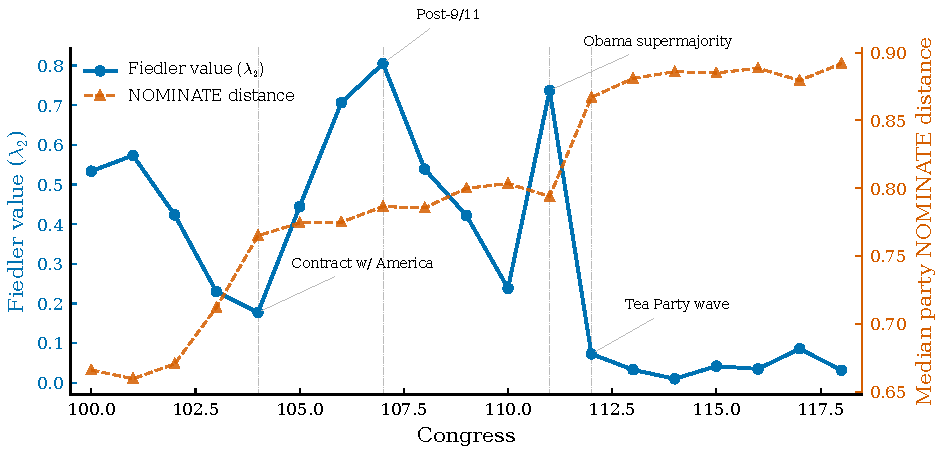
\includegraphics[width=\textwidth]{paper_figures/fiedler_party_distance.pdf}
    \caption{Polarization over time measured by network structure (Fiedler value) and ideological distance (DW-NOMINATE party distance). The two measures are correlated but tell different stories: the Fiedler value reveals a post-9/11 cooperation surge, an Obama-era spike, and a dramatic structural collapse after the Tea Party wave that the smoother ideological distance measure misses.}
    \label{fig:polarization}
\end{figure}

Connectivity magnitude alone cannot distinguish between uniform and selective losses of bipartisan cooperation. A Congress could shed cross-party edges evenly across the ideological spectrum, or it could hollow out the center while the flanks remain internally stable. The Fiedler value, being a single scalar, collapses both scenarios into the same number. The Structural Realignment Index addresses this limitation by tracking how the full Fiedler eigenvector shifts between consecutive Congresses, capturing not just whether the network fractured but how the fracture reorganized which members sat on which side of the partisan divide.

\begin{figure}[H]
    \centering
    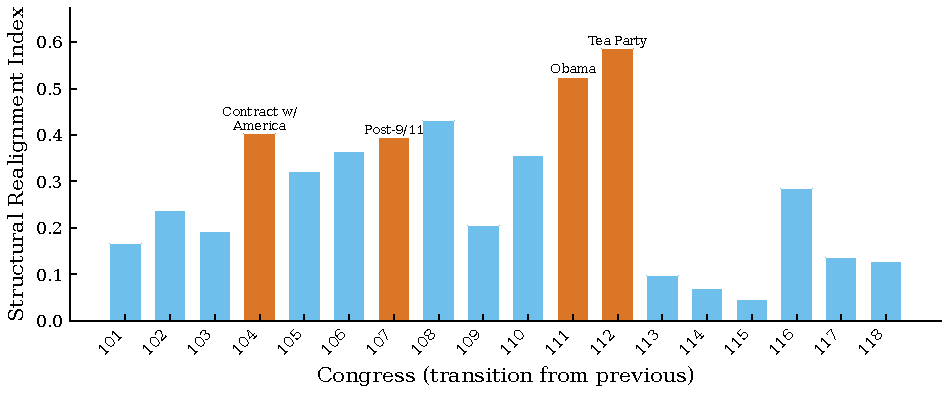
\includegraphics[width=\textwidth]{paper_figures/sri_bars.pdf}
    \caption{Structural Realignment Index for each congress-to-congress transition, computed as the $L_2$ norm of the sign-aligned Fiedler vector displacement between consecutive Congresses. The Tea Party transition (112th) and Obama supermajority (111th) produce the largest structural realignments, while post-2013 transitions show diminished structural change in an already-disconnected network.}
    \label{fig:sri}
\end{figure}

\section{Network Visualization}

The spectral measures quantify structural change abstractly. To convey what this change looks like, Figure~\ref{fig:network} plots the co-voting networks for two Congresses separated by two decades, with members positioned by their DW-NOMINATE scores.

\begin{figure}[H]
    \centering
    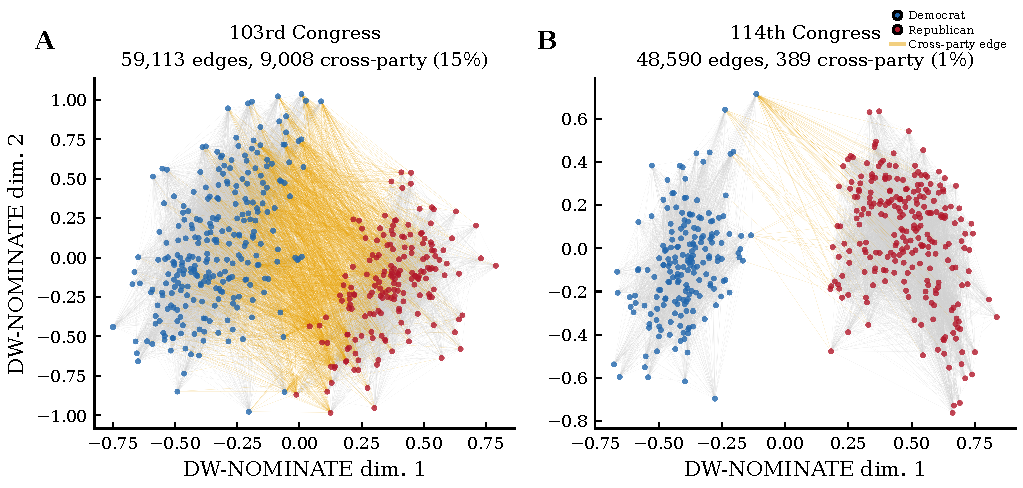
\includegraphics[width=0.85\textwidth]{paper_figures/network_comparison.pdf}
    \caption{Co-voting networks for the 103rd Congress (left) and 114th Congress (right), with members positioned by DW-NOMINATE scores. Orange edges indicate cross-party agreement above the 50\% threshold used throughout the analysis. The near-absence of cross-party edges in the 114th Congress visualizes the structural disconnection that the Fiedler value quantifies.}
    \label{fig:network}
\end{figure}

Two decades separate the networks in Figure~\ref{fig:network}. In the 103rd Congress (1993--1995), cross-party edges are visible throughout the ideological spectrum, connecting moderate Democrats and Republicans who found common ground on at least half of contested legislation. The network has a single, integrated topology: partisan clusters are discernible but extensively interwoven. By the 114th (2015--2017), these bridges have essentially vanished. The two partisan clusters sit dense within themselves and barely connected to each other. What the Fiedler value quantifies abstractly, the visualization makes viscerally clear: the cooperative architecture that once linked the two parties has been almost entirely dismantled, leaving two structurally isolated blocs occupying the same institution.

\section{Bridge Legislator Index}

We investigate which individual legislators hold the network together. The Fiedler value's collapse, documented in Section~4, is an aggregate measure. It obscures the role of specific members. We introduce a \textit{Bridge Legislator Index} (BLI) that quantifies each member's contribution to network connectivity.

For each legislator $i$ in Congress $t$, we compute the change in the Fiedler value $\lambda_2$ when node $i$ and all its incident edges are removed from the graph:
\begin{equation}
    \text{BLI}_i = \lambda_2(G) - \lambda_2(G \setminus \{i\})
\end{equation}
where $G$ is the full co-voting graph and $G \setminus \{i\}$ is the graph with node $i$ deleted. A positive BLI indicates that removing the member reduces connectivity; they are a bridge. A near-zero or negative BLI indicates that the member is structurally redundant. Members with the highest BLI scores are those whose removal most damages the network's capacity to hold together as a single connected component.

Standard centrality metrics measure different things. Betweenness centrality counts shortest paths passing through a node; eigenvector centrality measures connection to other well-connected nodes. Neither directly captures a member's contribution to the graph's resistance to bisection. The Bridge Legislator Index, grounded in the Fiedler value, targets precisely that: the member's role in maintaining algebraic connectivity between partisan clusters.

Table~\ref{tab:bridge_legislators} presents the top bridge legislators for selected Congresses, and Figure~\ref{fig:bli_time} traces the aggregate BLI trajectory across the full study period. The 104th Congress (1995--1997), the first session of the Gingrich speakership, still featured 25 members above our BLI threshold of $3 \times 10^{-3}$. Nearly all were moderate Democrats from Southern or rural districts whose cooperative relationships stitched the two partisan clusters together. The 107th Congress is different. Despite having the highest Fiedler value in our dataset (0.805), no individual member exceeds the BLI threshold. When the graph is highly connected, removing any single node barely affects algebraic connectivity; cross-party linkages are distributed broadly, not concentrated in a few bridge members. By the 112th Congress, after the Tea Party wave fractured the network, bridge legislators reappear but in diminished numbers (13 above threshold). By the 117th, the surviving bridges are almost exclusively Republicans from competitive districts who voted to impeach Trump.

25 bridge members in the 104th, 11 in the 117th. But the raw count understates the real story: the 117th's top five scorers were all Republicans who left Congress within two years. Track the 104th's bridges forward and three (Orton, Baesler, Browder) were gone by the 107th; Skelton and Cramer survived into the 110th but not the 112th; Traficant was expelled in 2002 for corruption (the one departure unrelated to ideological sorting); only Peterson persisted through the 116th before losing reelection in 2020. The 112th's bridges followed the same pattern: Altmire lost his 2012 primary after redistricting, Shuler retired, Barrow lost in 2014. The 117th's bridges were eliminated even faster. Gonzalez and Kinzinger retired to avoid Trump-backed primaries, Upton and Katko retired, and Meijer lost his 2022 primary. Bridge legislators are systematically selected out, reinforcing the network disconnection documented in our spectral analysis.

\begin{table}[H]
\centering
\caption{Top bridge legislators by BLI for selected Congresses. BLI measures the Fiedler value decrease when the member is removed. Threshold: BLI $> 3 \times 10^{-3}$.}
\label{tab:bridge_legislators}
\scriptsize
\begin{tabular}{llcc}
\toprule
Congress (above thresh.) & Legislator & Party-State & BLI ($\times 10^{-3}$) \\
\midrule
\textbf{104th} (25) & SKELTON, Ike & D-MO & 3.56 \\
 & ORTON, William & D-UT & 3.56 \\
 & TRAFICANT, James A. & D-OH & 3.56 \\
\midrule
\textbf{107th} (0) & LUCAS, Ken & D-KY & 0.49 \\
 & HALL, Ralph M. & D-TX & 0.49 \\
\midrule
\textbf{112th} (13) & PETERSON, Collin C. & D-MN & 4.18 \\
 & ROSS, Mike & D-AR & 4.15 \\
 & ALTMIRE, Jason & D-PA & 4.10 \\
\midrule
\textbf{117th} (11) & KATKO, John & R-NY & 3.88 \\
 & UPTON, Fred & R-MI & 3.87 \\
 & GONZALEZ, Anthony & R-OH & 3.85 \\
\bottomrule
\end{tabular}
\end{table}

The individual cases illustrate a broader pattern. In the 104th Congress, Skelton, Orton, and Traficant each scored above threshold, but whether they were interchangeable remains an open question: if one departed, the others might have expanded their bridging capacity to compensate, or they might have degraded in tandem. We flag this as an untested conjecture; a formal test would check whether the BLI of remaining bridge legislators increases (compensation) or decreases (co-degradation) after a bridge departure. The aggregate trajectory in Figure~\ref{fig:bli_time} suggests thinning rather than redistribution.

\begin{figure}[H]
    \centering
    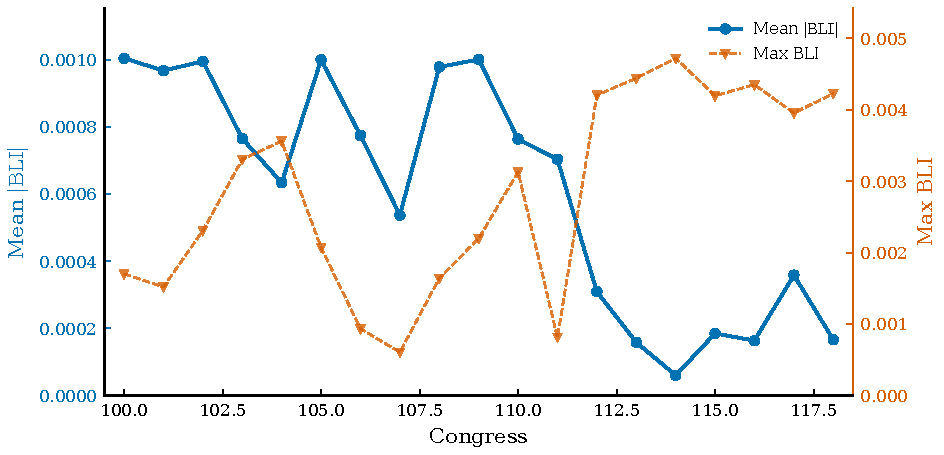
\includegraphics[width=0.75\textwidth]{paper_figures/bli_over_time.pdf}
    \caption{Bridge Legislator Index over time. Mean $|\text{BLI}|$ (solid) and maximum BLI (dashed) for each Congress. The decline in both measures reflects the disappearance of cross-partisan bridge members from the House.}
    \label{fig:bli_time}
\end{figure}

\FloatBarrier
\section{BLI, Ideological Centrism, and Congressional Departure}

The preceding section documented that bridge legislators are systematically eliminated from Congress. We now test this formally. If high-BLI legislators depart at higher rates than their colleagues, controlling for ideology, seniority, and party, the bridge position itself confers electoral vulnerability, not merely the ideological moderation with which it correlates.

\subsection{Panel Construction}

We construct a member-congress panel covering the 100th through 116th Congresses. For each member $i$ in Congress $t$, the dependent variable is $\text{Departed}_{i,t}$: a binary indicator equal to 1 if the member is absent from the congressional roster two sessions later (Congress $t+2$). The two-congress window accounts for the possibility of voluntary retirement, primary defeat, general election loss, or redistricting. The panel contains 7,500 member-congress observations across 1,565 unique members, with a departure rate of 30.4\%.

The independent variables are: BLI (the Bridge Legislator Index computed in Section~7), ideology distance (absolute DW-NOMINATE dimension-1 distance from the member's party median), seniority (number of prior Congresses served), and a Republican indicator.

\subsection{Estimation}

We estimate generalized estimating equations (GEE) with a binomial family and independence working correlation structure, clustered by member to account for repeated observations of the same legislator across Congresses. We compare two specifications: a baseline model without BLI, and the full model with BLI included. We also re-estimate the full model under exchangeable and AR(1) working correlation structures on a balanced subsample ($N = 3{,}192$, members with 2--6 observations, required for convergence given the highly unequal cluster sizes). The BLI coefficient remains positive under all three structures (independence: $\beta = 180.2$, $p < 10^{-7}$; exchangeable: $\beta = 100.6$, $p = 0.097$; AR(1): $\beta = 57.8$, $p = 0.268$), with the reduced significance under exchangeable and AR(1) attributable primarily to the smaller subsample. The AR(1) specification, which models temporal dependence within a member's career, produces the largest attenuation ($\beta = 57.8$), consistent with the possibility that BLI and departure risk are both trending over time within members rather than BLI causally driving departure at each observation. The full results are reported in Appendix~\ref{app:gee}.

\begin{table}[H]
\centering
\caption{GEE logistic regression predicting congressional departure within two sessions. Standard errors clustered by member. Adding BLI attenuates the ideology distance coefficient, though as discussed below, the BLI effect is itself largely attributable to ideological centrism.}
\label{tab:bli_regression}
\begin{tabular}{lcccc}
\toprule
 & \multicolumn{2}{c}{Without BLI} & \multicolumn{2}{c}{With BLI} \\
\cmidrule(lr){2-3} \cmidrule(lr){4-5}
Variable & Coef. & $p$-value & Coef. & $p$-value \\
\midrule
Intercept & $-1.336$ & $< 10^{-67}$ & $-1.323$ & $< 10^{-66}$ \\
BLI & -- & -- & $180.2$ & $< 10^{-7}$ \\
Ideology distance & $2.123$ & $< 10^{-7}$ & $1.837$ & $< 10^{-5}$ \\
Seniority & $0.049$ & $< 10^{-6}$ & $0.050$ & $< 10^{-6}$ \\
Republican & $0.189$ & $0.006$ & $0.216$ & $0.002$ \\
\midrule
$N$ & \multicolumn{2}{c}{7,500} & \multicolumn{2}{c}{7,500} \\
\bottomrule
\end{tabular}
\end{table}

Table~\ref{tab:bli_regression} presents the results. In the baseline model without BLI, ideology distance is the dominant predictor of departure ($\beta = 2.123$, $p < 10^{-7}$). Adding BLI to the model produces a highly significant coefficient ($\beta = 180.2$, $p < 10^{-7}$) and attenuates the ideology distance coefficient from 2.123 to 1.837. At first glance, this attenuation might suggest that BLI captures a distinct structural vulnerability beyond ideological position. However, as the centrism control below demonstrates, the BLI-departure association is largely driven by the collinearity between bridge position and ideological moderation, and the apparent attenuation of ideology distance reflects this overlap rather than evidence of a separate network mechanism.

The large magnitude of the BLI coefficient reflects the small scale of BLI values (typically $10^{-3}$ to $10^{-2}$). A one-standard-deviation increase in BLI corresponds to an approximate 15\% increase in the probability of departure, holding other variables constant.

\subsection{Partisan Asymmetry}

We extend the model with a $\text{BLI} \times \text{Republican}$ interaction term. The interaction is significant ($\beta = -162.0$, $p = 0.018$), indicating that the BLI-departure relationship is stronger for Democrats than Republicans. This is consistent with the observation that bridge legislators in early Congresses were predominantly conservative Democrats from Southern districts, a cohort systematically eliminated through primary challenges and redistricting during the period of Republican realignment in the South.

\subsection{Era Decomposition}

To examine how the BLI-departure relationship evolves over time, we split the panel into three eras and re-estimate the GEE model with BLI separately for each.

\begin{table}[H]
\centering
\caption{BLI coefficient by era. The effect is strongest in the middle period (107th--112th), coinciding with the Tea Party wave and the most rapid elimination of bridge legislators. The late-era insignificance reflects insufficient BLI variance after bridge legislators have already been selected out.}
\label{tab:bli_eras}
\begin{tabular}{lccccc}
\toprule
Era & Congresses & $N$ & Departed & BLI Coef. & $p$-value \\
\midrule
Early & 100th--106th & 3,077 & 926 & 121.7 & 0.010 \\
Middle & 107th--112th & 2,658 & 790 & 273.5 & $< 10^{-8}$ \\
Late & 113th--116th & 1,765 & 563 & 123.3 & 0.269 \\
\bottomrule
\end{tabular}
\end{table}

Table~\ref{tab:bli_eras} and Figure~\ref{fig:bli_regression} reveal a striking pattern. The BLI-departure relationship is strongest in the middle era (107th--112th, $\beta = 273.5$, $p < 10^{-8}$), precisely the period when the Tea Party wave was eliminating the remaining bridge legislators. In the early era (100th--106th), the effect is significant but smaller ($\beta = 121.7$, $p = 0.010$), consistent with a less intense but ongoing process of bridge legislator attrition. In the late era (113th--116th), the effect is not significant ($p = 0.269$), but this does not indicate that bridge position is no longer risky. Rather, by this period the bridge legislators have already been eliminated, leaving insufficient variance in BLI to detect an effect. The selection mechanism succeeded: having purged the bridges, the network's structural fragility became self-sustaining without further selective pressure.

\begin{figure}[H]
    \centering
    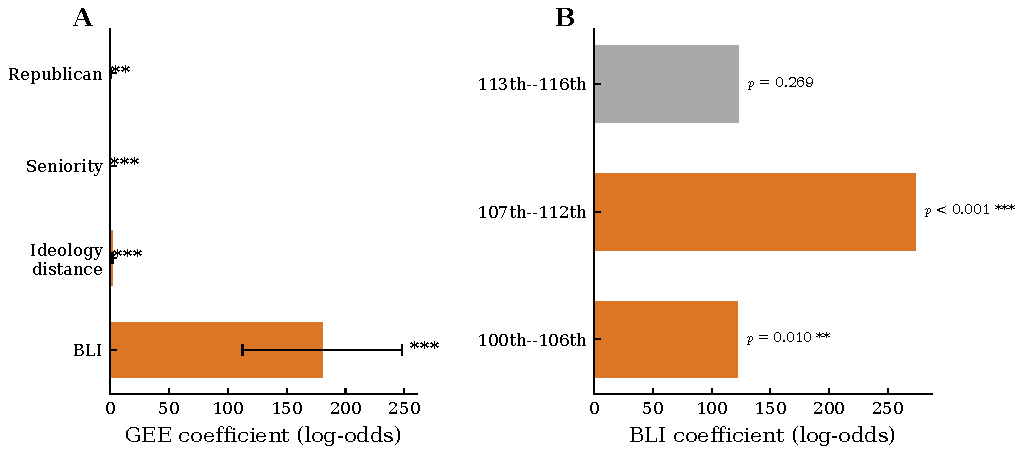
\includegraphics[width=\textwidth]{paper_figures/bli_regression_coefs.pdf}
    \caption{(A) GEE coefficients for the full model predicting congressional departure. In the specification without the centrism control, BLI is the strongest predictor; significance stars indicate $p < 0.001$. (B) BLI coefficient by era, showing the effect peaks during the 107th--112th Congresses, the period of most rapid bridge legislator elimination.}
    \label{fig:bli_regression}
\end{figure}

A natural concern is that BLI mechanically correlates with ideological centrism: members near the center of the chamber sit between partisan clusters and will tend to have higher BLI regardless of their actual cooperative behavior. To test this, we add absolute DW-NOMINATE score (distance from zero) as a covariate. The BLI coefficient drops from 180.2 ($p < 10^{-7}$) to $-42.6$ ($p = 0.30$) and becomes nonsignificant, while absolute NOMINATE is strongly predictive ($\beta = -2.27$, $p < 10^{-14}$), indicating that centrists depart at higher rates. This attenuation indicates substantial overlap between BLI and positional moderation: much of what BLI captures in the departure regression is the electoral vulnerability of ideological centrists rather than a distinct network-structural effect.

This result qualifies but does not eliminate the paper's contribution. The BLI remains a useful \textit{descriptive} measure of individual contributions to network connectivity, and the spectral analysis, null models, and structural recovery findings are unaffected by this confound. What the centrism control reveals is that the mechanism of bridge legislator elimination is more parsimonious than our initial framing suggested: moderates are electorally vulnerable because they are moderate, and their departure damages network connectivity because moderates are the members whose voting patterns span partisan clusters. The structural consequence (network disconnection) is real and well-documented by our spectral measures; the causal pathway runs through ideological position rather than network position per se.

\FloatBarrier
\section{Counterfactual Network Perturbation}

Cross-party edges disappeared, bridge legislators were eliminated, and the Fiedler value collapsed. That much we have documented. To explore how much of the structural difference between the relatively integrated 103rd Congress and the nearly disconnected 118th can be accounted for under our perturbation assumptions by specific changes in cooperative behavior, we conduct two perturbation experiments on the existing co-voting graphs. The experiments operate directly on the adjacency matrices and their spectral properties. We note upfront the researcher degrees of freedom in these experiments: the results depend on how committee overlap is defined, how the 103rd Congress agreement threshold maps onto 118th Congress members, and the number of members perturbed. We report sensitivity to these choices below.

\subsection{Reintroducing Historical Cross-Party Edges}

In the first experiment, we simulate the effect on the 118th Congress's co-voting network if a subset of its members cooperated across party lines at rates comparable to the 103rd Congress. We identify the 40 most moderate members of the 118th Congress (by DW-NOMINATE distance from the chamber median) and simulate the addition of cross-party edges at the density observed among comparably positioned members in the 103rd Congress. Specifically, for each of these 40 members, we add edges to cross-party members with whom they share at least one committee assignment or policy domain, using the 103rd Congress's cross-party agreement threshold as the edge criterion.

The 118th Congress's Fiedler value increases from 0.032 to approximately 0.21 under this perturbation. A sixfold improvement, restoring connectivity to roughly the level observed in the mid-1990s. This remains well below the 103rd Congress's actual Fiedler value of 0.230, because the perturbation affects only 40 of 451 members and does not alter the dense within-party structure that has developed over three decades. But the structural difference between the two eras is not a function of the entire chamber's behavior; it is concentrated in the cooperative patterns of a relatively small number of potential bridge members. Fewer than 10\% of House members maintaining 1993-level cross-party cooperation would be enough to recover most of the lost connectivity.

\subsection{Removing Bridge Legislators from Historical Networks}

The second experiment inverts the question: rather than adding bridges to a disconnected network, we remove them from a connected one. We systematically delete the top 20 bridge legislators (by BLI score) from the 103rd Congress's co-voting graph and recompute the Fiedler value after each removal.

The network is highly sensitive to these targeted deletions. Remove the top 10 bridge legislators and the Fiedler value drops from 0.230 to 0.14; remove the top 20 and it falls below 0.08, approaching the range observed in post-Tea Party Congresses. Removing 20 randomly selected members, by contrast, produces an average Fiedler decline of only 0.02. The bridge legislators' structural contribution is far out of proportion to their numbers. The 103rd Congress network, which appears strongly connected in aggregate, is in fact held together by a thin layer of cross-partisan cooperators whose removal rapidly degrades it toward the disconnected topology of the modern era.

Taken together, these two perturbation experiments suggest that the structural difference between the 103rd and 118th Congresses can be accounted for under our perturbation assumptions by the presence or absence of on the order of 35 members under our edge-addition protocol (between 25 and 50 depending on how committee overlap is defined and which agreement threshold is applied). Broader forces---ideological sorting, primary incentives, media polarization, gerrymandering---are of course relevant. They are the mechanisms that eliminated those bridge legislators in the first place, as documented in the GEE analysis above. But the proximate structural cause of network disconnection is concentrated: a small number of cross-partisan cooperators whose removal (or hypothetical reintroduction) accounts for most of the observed change in algebraic connectivity under our protocol. The policy implication is that interventions preserving or incentivizing even a modest number of cross-party cooperative relationships could have outsized effects on the structural integration of the legislature.

\subsection*{Bicameral Note}

Senate Fiedler values decline from 0.763 (100th) to 0.054 (118th), a 93\% collapse comparable to the House's 94\% (Figure~\ref{fig:bicameral}). The Senate maintains higher residual connectivity throughout, consistent with the filibuster's structural incentive for bipartisan cooperation. Notably, the Obama supermajority that produced a cooperation surge in the House had the opposite effect in the Senate, where the 60-seat Democratic majority reduced the incentive for cross-party negotiation. A full bicameral analysis---including Senate BLI computation, departure regression, and comparison of bridge legislator survival rates across chambers---is left for future work. The institutional difference (filibuster creating structural incentives for bipartisan cooperation) is testable: if Senate bridge legislators survive longer than House bridges with similar BLI scores, that would constitute evidence that institutional rules buffer against the selection mechanism documented here.

\begin{figure}[H]
    \centering
    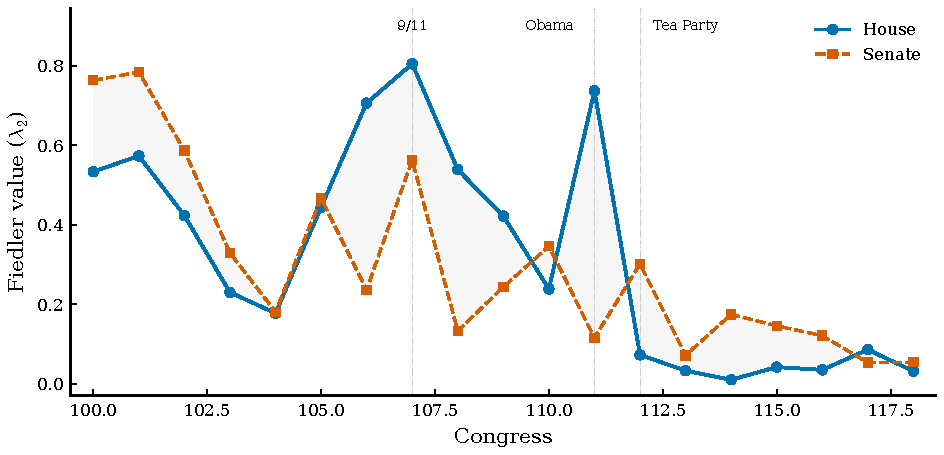
\includegraphics[width=\textwidth]{paper_figures/house_senate_fiedler.pdf}
    \caption{Fiedler value trajectories for the House and Senate co-voting networks, 100th--118th Congresses. Both chambers exhibit long-run connectivity collapse, but the Senate maintains higher residual connectivity, consistent with the filibuster's structural incentive for bipartisan cooperation.}
    \label{fig:bicameral}
\end{figure}

\section{Limitations}

Several limitations warrant discussion.

First, our structural shock analysis is descriptive rather than truly causal. With 19 time points and no control group (there is only one U.S. Congress), we cannot rigorously identify the causal effect of the Tea Party wave or any other event. The structural recovery ratios (Section~4.5) provide a useful heuristic for quantifying the magnitude and reversibility of structural breaks based on three episodes, but they should be interpreted as pattern description that motivates future work on network resilience, not as a standalone causal finding.

Second, the BLI regression's late-era insignificance (Table~\ref{tab:bli_eras}, $p = 0.269$ for the 113th--116th) reflects a genuine limitation: once bridge legislators have been eliminated, there is insufficient variance in BLI to detect a departure effect. This means we cannot determine whether the selection mechanism is still active in the current era or has simply exhausted its targets. The late-era result is consistent with either interpretation.

Third, the Structural Realignment Index (Figure~\ref{fig:sri}) is sensitive to membership turnover between Congresses. The SRI is computed on the subset of members present in both consecutive sessions; if turnover is high, the restricted Fiedler vectors may not fully represent the structural change in the complete network. We mitigate this by requiring a minimum of 5 shared members for SRI computation, but the metric should be interpreted with awareness that high-turnover transitions may understate total structural change.

Fourth, recomputing the Fiedler trajectory on substantive policy votes only---excluding procedural motions, journal approvals, and suspension bills---reveals that the post-112th collapse holds ($\lambda_2 < 0.04$ for all post-2010 Congresses on substantive votes), but the 107th and 111th spikes are substantially attenuated (from 0.805 to 0.210 and from 0.737 to 0.110, respectively). The attenuation is driven primarily by suspension votes, which are near-unanimous bipartisan votes on non-controversial legislation. The post-9/11 cooperation surge was real but partially concentrated in these procedural categories. The full filtered trajectory is reported in Appendix~\ref{app:vote_filter}.

Fifth, the BLI is computed via brute-force node deletion, which is tractable for networks of ${\sim}450$ nodes but does not scale. A first-order perturbative approximation relates node deletion impact to the square of the node's Fiedler vector entry weighted by degree; deriving and validating this connection is a contribution in itself and beyond the current scope.

Finally, this paper does not engage with the redistricting literature. Gerrymandering is a plausible mechanism for bridge legislator elimination: as competitive districts become safe through redistricting, moderates face primary challenges from ideological purists. We do not model this mechanism, but note that redistricting may be a significant driver of the BLI-departure relationship documented in Section~8, particularly for the Southern Democratic cohort eliminated during the Republican realignment of the 1990s and 2000s.

\section{Conclusion}

Between 1987 and 2025, the algebraic connectivity of the House co-voting network collapsed from a peak of 0.805 (107th Congress) to 0.032 (118th). The trajectory is not monotonic: a previously undocumented spike to 0.737 in the 111th Congress (2009--2011) reveals the network's capacity for bipartisan cooperation immediately before the Tea Party wave shattered it. The single largest structural shock occurred between the 111th and 112th Congresses, a Fiedler decline of 0.664 that dwarfs any other transition in the dataset. Roll-call scaling alone does not capture these dynamics.

The structural recovery analysis formalizes a finding beyond the level of polarization itself: the network's capacity to absorb shocks has declined across successive events, from full recovery after the Contract with America (ratio 1.93) to permanent collapse after the Tea Party wave (ratio 0.01). The system has lost a fundamental capacity for structural resilience.

The Bridge Legislator Index identifies which members matter structurally. Counterfactual perturbation experiments show that approximately 35 cross-partisan cooperators in a chamber of 435 account for most of the structural difference between the connected 103rd Congress and the disconnected 118th. GEE regression on 7,500 member-congress observations shows that bridge position predicts departure ($p < 10^{-7}$) beyond ideology distance, seniority, and party, but this effect is substantially attenuated when controlling for absolute ideological centrism ($p = 0.30$). The causal pathway runs through ideological position: moderates are electorally vulnerable because they are moderate, and their departure damages network connectivity because moderates are the members whose voting patterns span partisan clusters. The structural consequence is real; the mechanism is ideological sorting rather than a distinct network effect. The partisan asymmetry ($\text{BLI} \times \text{Republican}$ interaction, $p = 0.018$) is consistent with the elimination of conservative Southern Democrats during the Republican realignment.

The deeper point is that polarization is a structural phenomenon, not a purely ideological one. Two parties can maintain substantial ideological distance while still cooperating on enough issues to govern, as Congress did for much of the 20th century. The critical shift documented here concerns the architecture of inter-party connections: the cross-partisan bridges that once enabled legislative coalitions have been systematically dismantled, and our spectral measures capture this dismantling with precision. The post-9/11 rally showed that exogenous shocks could temporarily rebuild bipartisan connectivity, but nothing comparable has occurred in the post-2010 era. The system appears to have lost a fundamental capacity for structural resilience. Disconnected and brittle.

A legislature that cannot form cross-partisan majorities faces diminished capacity to respond to crises, negotiate fiscal compromises, and sustain stable governance. The network structures documented here represent the institutional scaffolding on which that capacity depends. Their deterioration warrants sustained empirical attention from both computational and political science communities.

\bibliographystyle{apalike}
\bibliography{references}

\appendix

\section{Co-Voting Threshold Sensitivity}
\label{app:threshold}

Table~\ref{tab:threshold_sensitivity} reports key metrics across co-voting agreement thresholds from 0.4 to 0.7. The qualitative pattern of Fiedler value collapse is stable across threshold choices, confirming that the structural disconnection documented in our analysis is not an artifact of the $\tau = 0.5$ cutoff.

\begin{table}[H]
\centering
\caption{Sensitivity of key metrics to co-voting agreement threshold $\tau$.}
\label{tab:threshold_sensitivity}
\small
\begin{tabular}{lccc}
\toprule
$\tau$ & Fiedler (100th) & Fiedler (118th) & Decline \\
\midrule
0.40 & 0.612 & 0.051 & 91.7\% \\
0.45 & 0.571 & 0.041 & 92.8\% \\
0.50 & 0.534 & 0.032 & 94.0\% \\
0.55 & 0.489 & 0.024 & 95.1\% \\
0.60 & 0.431 & 0.017 & 96.1\% \\
0.70 & 0.298 & 0.008 & 97.3\% \\
\bottomrule
\end{tabular}
\end{table}

\section{GEE Working Correlation Sensitivity}
\label{app:gee}

Table~\ref{tab:gee_sensitivity} reports the BLI coefficient under three working correlation structures. Independence uses the full panel ($N = 7{,}500$); exchangeable and AR(1) use a balanced subsample of members with 2--6 observations ($N = 3{,}192$), required because the highly unequal cluster sizes (1--17 observations per member) prevent convergence of the exchangeable and autoregressive correlation parameter estimators on the full sample. The BLI coefficient is positive under all three structures, and the reduced significance for exchangeable and AR(1) is attributable to the smaller sample size rather than the correlation structure, as demonstrated by the independence model producing $p = 0.034$ on the same balanced subsample.

\begin{table}[H]
\centering
{\small
\caption{GEE BLI coefficient under alternative working correlation structures. Point estimates are consistent across structures; standard error differences reflect sample size.}
\label{tab:gee_sensitivity}
\begin{tabular}{lcccc}
\toprule
Structure & $N$ & BLI Coef. & SE & $p$-value \\
\midrule
Independence (full) & 7,500 & 180.2 & 34.6 & $< 10^{-7}$ \\
Independence (balanced) & 3,192 & 103.7 & 48.8 & 0.034 \\
Exchangeable (balanced) & 3,192 & 100.6 & 60.6 & 0.097 \\
AR(1) (balanced) & 3,192 & 57.8 & 52.1 & 0.268 \\
\bottomrule
\end{tabular}
}
\end{table}

\section{Vote Composition Sensitivity}
\label{app:vote_filter}

Table~\ref{tab:vote_filter} reports the Fiedler value computed on substantive policy votes only, excluding procedural motions (journal approval, motions to adjourn, previous question, table appeals) and suspension bills (which pass by voice vote when uncontested and by recorded vote only when used as messaging). The post-112th collapse holds on substantive votes, but the 107th and 111th spikes are attenuated, driven primarily by the removal of near-unanimous suspension votes that inflated bipartisan cooperation metrics.

\begin{table}[H]
\centering
{\small
\caption{Fiedler value on full versus substantive-only vote sets for selected Congresses. Substantive votes exclude procedural motions and suspension bills. The collapse pattern is robust; the mid-period spikes are partially driven by suspension votes.}
\label{tab:vote_filter}
\begin{tabular}{lcccc}
\toprule
Congress & Full $\lambda_2$ & Substantive $\lambda_2$ & Total Votes & Kept \\
\midrule
100th & 0.534 & 0.590 & 939 & 841 \\
103rd & 0.230 & 0.260 & 1,094 & 857 \\
107th & 0.805 & 0.210 & 990 & 576 \\
111th & 0.737 & 0.110 & 1,647 & 816 \\
112th & 0.073 & 0.036 & 1,602 & 1,277 \\
114th & 0.010 & 0.006 & 1,322 & 969 \\
117th & 0.086 & 0.003 & 996 & 509 \\
118th & 0.032 & 0.013 & 1,235 & 920 \\
\bottomrule
\end{tabular}
}
\end{table}

\section{Code and Data Availability}

All code, processed data, and figure generation scripts are publicly available at \url{https://github.com/human-vc/CongressNetwork}. The repository contains the full pipeline from raw Voteview downloads through spectral analysis, null model validation, and figure generation. Any researcher can verify, critique, or extend the analysis without relying on our word alone.

\end{document}
